\section{Fractional Differential Equations (FDEs)}
Differential equations involving fractional differential operators
have recently proved to be valuable tools in the modeling of many
physical phenomena.

We will focus our analysis in this section on FDEs of the Caputo type of the form
\begin{equation}
    \leftindex[I]^C {D^{\alpha}} y(t) = f(t,y(t))
\end{equation}
And some parts will deal with a slightly more general class of problems
then we will look into some of the methods to solve linear and nonlinear FDEs

The reason why we will use the Caputo derivative that RL fractional derivative $D^\alpha$ 
in order to obtain a particular solution to the straightforward form of a FDE
\[
    D^\alpha y(t) = f(t,y(t))
\]
We need to specify $m$ initial conditions corresponding to it and it must be of the form
\[
    \left[D^{\alpha-k} y(t)\right]_{t=0} = \beta_k \quad,\quad k = 1,2,\dots,m
\]
With given values $\beta_k$. Thus we are forced to specify some fractional derivatives
of the function $y$. In practical applications, these values are frequently
not available, and it may not even be clear what their physical meaning is

Therefore Caputo has suggested that one should incorporate the classical derivatives 
(of integer order) of the function $y$, as they are commonly used in initial value problems 
with integer order equations, into the fractional order equation, using the relation between RL and Caputo derivatives
\[
    \leftindex[I]^C {D^{\alpha}} y(t) = D^\alpha (y-T_{m-1}[y])
\]
Where $T_{m-1}[y]$ is the Taylor polynomial of order $m-1$ for $y$, centered at
$0$. Then, one can specify the initial conditions in the classical form
\[
    y^{(k)}(0) = \beta_k \quad,\quad k=0,1,2,\dots,m-1 
\]

In the classical theory of integer order ordinary differential equations, it is well
known that unique solutions can only be expected if the differential equation is accompanied by certain additional conditions. 
The same observation is true in the fractional case. The question is then where on the $t-axis$ such condition(s) should be imposed.

By choosing the differential operator starting point, that is, the point $0$ we have answered this question. 
Interpreting the free variable $t$ as a time variable,
this amounts to providing information at the beginning of the process that the
differential equation describes and to seeking the process behavior for times that are
in the future of this instant.

\subsection{Initial Value Problems For Single Term Equations}
We will study IVPs in the form (6.1)
Since exactly one differential operator occurs in this equation, this type of
equations is known as a single term FDE.

Thus the IVP will be in the form 
\begin{equation}
    \begin{cases}
        \leftindex[I]^C {D^{\alpha}} y(t) = f(t,y(t))
        \\
        I.C \Longrightarrow y^{(k)}(0) = \beta_k \quad,\quad k=0,1,2,\dots,m-1 
    \end{cases}
\end{equation}
We can Consider the classical theory as a special case. 
Many (but not all) classical results (and their proofs) can be generalized to this fractional setting

Almost all results are formulated for $d$-dimensional systems of equations 
with arbitrary $d \in \mathbb{N}$, that is, we assume the function $y(t)$ is vector valid function map an
interval $[0, T]$ to $\mathbb{R}^d$. Consequently, the initial values $\beta_k$ are vectors in $\mathbb{R}^d$, and the
function $f$ is assumed to map a subset of $[0, T]\times\mathbb{R}^d$ to $\mathbb{R}^d$.

\subsubsection{Existence And Uniqueness Of Solutions}
The most important results in the classical theory, Peano's existence theorem and the
Picard-Lindelöf uniqueness theorem, remain valid in the fractional setting too. Their
proofs are based on an equivalence between the IVP and a Volterra
integral equation. 

\begin{lemma}
Consider the IVP (6.2) and assume that the function $f := [0, T]\times\mathbb{R}^d \to \mathbb{R}^d$
with some $T > 0$ is continuous. Then the function $y(t) \in C[0, T]$ is a solution of
this IVP if and only if it is a solution of the nonlinear Volterra integral equation of the second kind
\[
    y(t) = \sum_{k=0}^{m-1} \frac{t^k}{k!} y^{(k)}(0) + \frac{1}{\Gamma(\alpha)} \int_{0}^{t} (t-s)^{\alpha-1}f(s,y(s)) \hquad ds
\]
\end{lemma}
\begin{proof}[Proof]
    let $\mathcal{L}[y(t)] = Y(s)$ be the Laplace transform of $y(t)$ then by taking Laplace transform for the equation in (6.2)
    we get 
    \begin{align*}
        s^{\alpha}Y(s) - \sum_{k=0}^{m-1} s^{\alpha-k-1} y^{(k)}(0) &= \mathcal{L}[f(t,y(t))]
        \\
        s^{\alpha}Y(s) - \sum_{k=0}^{m-1} s^{\alpha-k-1} \beta_k &= \mathcal{L}[f(t,y(t))]
        \\
        Y(s) &= \sum_{k=0}^{m-1} \frac{\beta_k}{s^{k+1}} + \frac{1}{s^{\alpha}}\mathcal{L}[f(t,y(t))]
        \\
        Y(s) &= \sum_{k=0}^{m-1} \frac{\beta_k}{s^{k+1}} + \mathcal{L}[I^{\alpha}f(t,y(t))]
        \intertext{Take Laplace inverse for both sides}
        y(t) &= \sum_{k=0}^{m-1} \frac{t^k}{k!} \beta_k + \frac{1}{\Gamma(\alpha)}\int_{0}^{t} (t-s)^{\alpha-1}f(s,y(s)) \hquad ds
    \end{align*}
\end{proof}
Based on this result, it is possible to prove using Schauder's fixedpoint
theorem the fractional analogue of Peano's existence theorem: Continuity and
boundedness of the given function $f$ on the right hand side suffice to assert the existence 
of a continuous solution to the IVP (6.2).
\begin{theorem}[Peano's Existence Theorem]
    $ $ \newline
    Let $0 \leq m-1 < \alpha < m $ and let $y(0),y^{(1)}(0),\dots,y^{(m-1)}(0) \in \mathbb{R}^d $ , $\eta>0,K>0$ 
    \\
    Consider the domain
    \\(a) $D := [0, \eta]\times\mathbb{R}^d$
    \\(b) $\displaystyle D := \left\{ (t,y) : t \in [0, \eta] \quad,\quad \left|\left| y-\sum_{k=0}^{m-1} \frac{t^k}{k!} y^{(k)}(0) \right|\right| \leq K \quad i.e \quad y \in \mathcal{N}_K(Initial \hquad points) \right\} $
    \\
    And that $f := D \to \mathbb{R}^d$ is continuous and bounded, with $M := \sup\limits_{(t,y)\in D} |f(t,y)|$. Moreover , let
    \begin{equation}
        \delta := \begin{cases}
            \eta     & \text{\textit{if M=0 or D = $[0, \eta]\times\mathbb{R}^d$}}
            \\
            \displaystyle \min\left\{\eta , \left(\frac{K\Gamma(\alpha+1)}{M}\right)^{\frac{1}{\alpha}} \right\} &\text{else}
        \end{cases}
    \end{equation}
    Then there exists a function $y(t) \in C[0, \delta]$ solves the IVP (6.2).
\end{theorem}

Note that the set $D$ is compact in case (b). Hence, in this case the boundedness of
$f$ on $D$ is an immediate consequence of it's continuity and does not need to be shown
explicitly.
Theorem (6.2) only guarantee the existence to get the uniqueness consider the following

The classical Picard-Lindelöf theorem can be generalized to the fractional setting
in the same way: If the given function $f$ is continuous and bounded and satisfies 
a Lipschitz condition with respect to the second variable, then uniqueness of the 
continuous solution to the IVP (6.2) can be guaranteed.

\begin{theorem}[Picard-Lindelöf Uniqueness Theorem]
    Assume the hypotheses of Theorem (6.2). Moreover, let $f$ fulfill a Lipschitz condition with respect to the second variable,
    that is,
    \[
        \left|\left| f(t,y_1)-f(t,y_2) \right|\right| \leq L \left|\left| y_1-y_2 \right|\right|
    \]
    Where $L$ is Lipschitz constant Then there exists a uniquely defined function $y(t) \in C[0, \delta]$ solves the IVP (6.2) where
    $\delta$ is given according to (6.3)
\end{theorem}
\begin{proof}[Proof (6.2)(6.3)]
    We consider the Voltera integral from Lemma (6.1)
    \[
        y(t) = \sum_{k=0}^{m-1} \frac{t^k}{k!} y^{(k)}(0) + \frac{1}{\Gamma(\alpha)} \int_{0}^{t} (t-s)^{\alpha-1}f(s,y(s)) \hquad ds
    \]
    Using the method of successive approximations we will prove the existence and the uniqueness of the solution of Caputo FDE.
    \[
        y_n(t) = \sum_{k=0}^{m-1} \frac{t^k}{k!} y^{(k)}(0) + \frac{1}{\Gamma(\alpha)} \int_{0}^{t} (t-s)^{\alpha-1}f(s,y_{n-1}(s)) \hquad ds
    \]
    For the sequence $\{y_n(t)\}$, we need to prove that:
    \begin{enumerate}[label=\roman*.]
        \item The sequence $\{y_n(t)\}$ is well defined
        \item The sequence is uniformly convergent
        \item And it's limit $y(t)$ is unique
    \end{enumerate}
    \begin{proof}[Proof (i)]
        We will use the induction method. 
        
        In the case $n = 0$ it is obvious.
        \[
            y_0(t) = \sum_{k=0}^{m-1} \frac{t^k}{k!} \beta_k
        \]
        If $n = 1$, then we have:
        \begin{align*}
            |y_1(t)-y_0(t)| &= \left| \frac{1}{\Gamma(\alpha)} \int_{0}^{t} (t-s)^{\alpha-1}f(s,y_{0}(s)) \hquad ds \right|
            \\
            &\leq \frac{1}{\Gamma(\alpha)} \int_{0}^{t} \left|(t-s)^{\alpha-1}\right|\left|f(s,y_{0}(s))\right| \hquad ds 
            \intertext{Because $M := \sup\limits_{(t,y)\in D} |f(t,y)|$}
            &\leq \frac{M}{\Gamma(\alpha)} \int_{0}^{t} (t-s)^{\alpha-1} \hquad ds 
            \\
            &\leq \frac{M}{\Gamma(\alpha)}\frac{t^\alpha}{\alpha}
            \intertext{Also because $t \in [0,\delta]$}
            &\leq \frac{M\delta^\alpha}{\Gamma(\alpha+1)} < \eta 
        \end{align*}
        If we assume 
        \[
            |y_{n-1}(t)-y_0(t)| < \eta 
        \]
        Then it follows that
        \begin{align*}
            |y_n(t)-y_0(t)| &= \left| \frac{1}{\Gamma(\alpha)} \int_{0}^{t} (t-s)^{\alpha-1}f(s,y_{n-1}(s)) \hquad ds \right|
            \\
            &\leq \frac{M}{\Gamma(\alpha)} \int_{0}^{t} (t-s)^{\alpha-1} \hquad ds 
            \\
            &\leq \frac{M}{\Gamma(\alpha)}\frac{t^\alpha}{\alpha}
            \\
            &\tag{$\circledast$} \leq \frac{M\delta^\alpha}{\Gamma(\alpha+1)} < \eta 
        \end{align*}
    \end{proof}
    \begin{proof}[Proof (ii)]
        From $(\circledast)$ we can deduce the relation 
        \[
            \frac{\delta^\alpha}{\Gamma(\alpha+1)} \leq \frac{\eta}{M}
        \]
        Now 
        \begin{align*}
            |y_2(t)-y_1(t)| &= \left| \frac{1}{\Gamma(\alpha)} \int_{0}^{t} (t-s)^{\alpha-1}\left[f(s,y_{1}(s))-f(s,y_{0}(s))\right] \hquad ds \right|
            \\
            &\leq \frac{L}{\Gamma(\alpha)} \int_{0}^{t} (t-s)^{\alpha-1} \left|y_1-y_0\right| \hquad ds 
            \\
            &\leq \frac{L\eta}{\Gamma(\alpha)} \int_{0}^{t} (t-s)^{\alpha-1} \hquad ds 
            \\
            &\leq \frac{L\eta}{\Gamma(\alpha)} \frac{t^\alpha}{\alpha}
            \\
            &\leq \frac{L\eta\delta^\alpha}{\Gamma(\alpha+1)} <  \frac{L\eta^2}{M}
        \end{align*}
        \begin{align*}
            |y_3(t)-y_2(t)| &= \left| \frac{1}{\Gamma(\alpha)} \int_{0}^{t} (t-s)^{\alpha-1}\left[f(s,y_{2}(s))-f(s,y_{1}(s))\right] \hquad ds \right|
            \\
            &\leq \frac{L}{\Gamma(\alpha)} \int_{0}^{t} (t-s)^{\alpha-1} \left|y_2-y_1\right| \hquad ds 
            \\
            &\leq \frac{L^2\eta^2}{M\Gamma(\alpha)} \int_{0}^{t} (t-s)^{\alpha-1} \hquad ds 
            \\
            &\leq \frac{L^2\eta^2}{M\Gamma(\alpha)} \frac{t^\alpha}{\alpha}
            \\
            &\leq \frac{L^2\eta^2\delta^\alpha}{M\Gamma(\alpha+1)} < \frac{L^2\eta^3}{M^2}
        \end{align*}
        And so on we get 
        \[
            |y_{n+1}(t)-y_{n}(t)| \leq \eta \left(\frac{L\eta}{M}\right)^{n}
        \]
        Now summing over $n$ to get the solutions
        \[
            y_{0}(t) + \sum_{k=0}^{n} y_{k+1}(t)-y_{k}(t) = y_{0}(t) + y_{n+1}(t)-y_{n}(t)+y_{n}(t)-\dots-y_{0}(t) = y_{n+1}(t)
        \]
        Take the limit as $n \to \infty$ we get 
        \begin{align*}
            \lim_{n \to \infty} y_{n+1}(t) &= y_{0}(t) + \lim_{n \to \infty} \sum_{k=0}^{n} y_{k+1}(t)-y_{k}(t)
            \\
            y(t) &= y_{0}(t) + \sum_{k=0}^{\infty} y_{k+1}(t)-y_{k}(t)
        \end{align*}
        Using Weierstrass Test 
        \[
            \sum_{k=0}^{\infty} |y_{k+1}(t)-y_{k}(t)| \leq \eta \sum_{k=0}^{\infty} \left(\frac{L\eta}{M}\right)^{k}
        \]
        Thus The series are convergent if $\displaystyle \eta < \frac{M}{L}$

        Thus the sequence $\{y_n(t)\}$ is uniform convergent on the compact $[0, \eta]$.
        Hence, $y_n(t)$ is convergent to a function $y(t)$ for $t \in [0, \eta]$.
        \[
            \forall \eta >0 , \exists N>0 \text{ such that } \forall n>N \Longrightarrow |y_n(t) - y(t)| < \eta
        \]
    \end{proof}
    \begin{enrichment*}{The Weierstrass Test}
        Suppose that $\{f_n(t)\}$ is a sequence of real functions defined on a set $A$, 
        and there is a sequence of positive numbers $\{R_n\}$ satisfying:
        \[
            \forall n > 0 , \forall t \in A \quad,\quad |f_n(t)|<R_n \quad,\quad \sum_{n=0}^{\infty} R_n < \infty
        \]
        Then the series
        \[
            \sum_{n=0}^{\infty} f_n(t)
        \]
        Is convergent
    \end{enrichment*}
    \begin{proof}[Proof (iii)]
        $ $\newline 
        Let $x(t)$ be another limit for $\{y_n(t)\}$, then:
        \[
            |x(t)-y(t)| = |x(t)-y_n(t)+y_n(t)-y(t)| \leq |x(t)-y_n(t)|+|y_n(t)-y(t)| \leq \frac{\eta}{2}+\frac{\eta}{2} = \eta
        \]
    \end{proof}
\end{proof}
\newpage
\begin{example}
    Test the existence and uniqueness and find the possible values for $\alpha$ such that the equation has a unique solution
    \[
        \begin{cases}
            \leftindex[I]^C {D^{\alpha}} y(t) = t^2 + y^2 \quad,\quad 0< \alpha \leq 1 \quad,\quad (t,y) \in [-1,1]\times[-1,1]
            \\
            I.C \Longrightarrow y(0) = 0
        \end{cases}
    \]
    \textit{ \textbf{Sol.} } First
    \[
    M := \sup\limits_{(t,y)\in D} |f(t,y)| = f(1,1) = 2
    \]
    Now for the Lipschitz constant $L$
    \begin{align*}
        ||f(t,y_1)-f(t,y_2)|| &= ||t^2+y_1^2-t^2-y_2^2||
        \\
        &= ||y_1^2-y_2^2||
        \\
        &= ||(y_1+y_2)(y_1-y_2)||
        \\
        &\leq ||(1+1)(y_1-y_2)|| = 2||(y_1-y_2)||
    \end{align*}
    And 
    \begin{align*}
        \eta &= \min\left\{\eta , \left(\frac{K\Gamma(\alpha+1)}{M}\right)^{\frac{1}{\alpha}} \right\}
        \\
        &= \min\left\{1 , \left(\frac{1\times \Gamma(\alpha+1)}{2}\right)^{\frac{1}{\alpha}} \right\}
    \end{align*}
    We want 
    \[
        \eta < \frac{M}{L} = \frac{2}{2} = 1
    \]
    Thus the following must be true
    \begin{align*}
        \left(\frac{\Gamma(\alpha+1)}{2}\right)^{\frac{1}{\alpha}} &< 1
        \\
        \Gamma(\alpha+1) &< 2
    \end{align*}
    Because $0< \alpha \leq 1$ Thus it holds for any value of $\alpha$

    Thus equation has a unique solution

    And for $0< \alpha < 2$ this statement is true
    % \\
    % now to find it's solution
    % \[
    %     y_n(t) = \frac{1}{\Gamma(\alpha)}\int_{0}^{t} (t-s)^{\alpha-1}\left[s^2 + y_{n-1}^2\right]ds
    % \]
    % \begin{align*}
    %     y_0 &= 0
    %     \\
    %     y_1 &= \frac{1}{\Gamma(\alpha)}\int_{0}^{t} (t-s)^{\alpha-1}s^2ds
    %     \intertext{The Laplace transform of this convolution is}
    %     Y_1 &= \frac{1}{\Gamma(\alpha)} \frac{\Gamma(\alpha)}{s^{\alpha}}\frac{\Gamma(3)}{s^{3}} = \frac{2}{s^{\alpha+3}}
    %     \intertext{using inverse Laplace transform}
    %     y_1 &= \frac{2 t^{\alpha+2}}{\Gamma(\alpha+3)}
    %     \intertext{Similarly, we obtain also:}
    %     y_2 &= \frac{1}{\Gamma(\alpha)} \int_{0}^{t} (t-s)^{\alpha-1}\left[s^2 + \frac{4 t^{2\alpha+4}}{\Gamma^2(\alpha+3)}\right]ds
    %     \\
    %     Y_2 &= \frac{2}{s^{\alpha+3}} + \frac{4}{\Gamma^2(\alpha+3)} + \frac{\Gamma(2\alpha+5)}{s^{3\alpha +5}}
    %     \\
    %     y_2 &= \frac{2 t^{\alpha+2}}{\Gamma(\alpha+3)} + \frac{4 t^{3\alpha +4 }}{\Gamma^2(\alpha+3)} \frac{\Gamma(2\alpha+5)}{\Gamma(3\alpha+5)}
    %     \intertext{and so on}
    %     y_3 &= \frac{2 t^{\alpha+2}}{\Gamma(\alpha+3)} 
    %         + \frac{4 t^{3\alpha +4 }}{\Gamma^2(\alpha+3)} \frac{\Gamma(2\alpha+5)}{\Gamma(3\alpha+5)}
    %         + \frac{16 t^{7\alpha +8 }\Gamma^2(2\alpha+5)}{\Gamma^4(\alpha+3)\Gamma^2(3\alpha+5)} \frac{\Gamma(6\alpha+9)}{\Gamma(7\alpha+9)}
    % \end{align*}
\end{example}
\begin{example}
    Consider the following IVP
    \begin{equation}
        \begin{cases}
            \leftindex[I]^C {D^{\alpha}} y(t) = (y(t))^\mu
            \\
            I.C \Longrightarrow y(0) = 0
        \end{cases}
    \end{equation}
    With arbitrary $ 0< \alpha \leq 1$ and $ 0<\mu<1$ does not satisfy the Lipschitz condition mentioned
    in Theorem (6.3). Since it has the solutions
    \[
        y(t) = 0 \quad \text{and} \quad y(t) = \left( \frac{\Gamma\left(\frac{\alpha}{1-\mu}+1-\alpha\right)}{\Gamma\left(\frac{\alpha}{1-\mu}\right)}  \right)^{\frac{1}{1-\mu}} t^{\frac{\alpha}{1-\mu}}
    \]
\end{example}
It shows that the Lipschitz condition is a necessary condition for the uniqueness.
However, it is possible to recover the uniqueness if the Lipschitz condition is replaced
by a different suitable condition. For a one dimensional problem, a possible
choice in the case $0 < \alpha < 1$ that is also known from the classical theory is Nagumo's condition.
\begin{theorem}[Nagumo's Uniqueness Theorem]
    Let $\alpha \in (0, 1), T > 0$ and $y(0) \in \mathbb{R}$. If the function 
    $f := [0, T] \times \mathbb{R} \to \mathbb{R}$ is continuous at $(0, y(0))$ and satisfies the inequality
    \[
        t^\alpha |f(t,y_1)-f(t,y_2)| \leq \Gamma(\alpha+1)|y_1-y_2| \quad,\quad \forall t \in [0,T] \text{ and } \forall y_1,y_2 \in \mathbb{R}
    \]
    Then the IVP (6.2) has at most one continuous solution $y$ on $[0, T]$ satisfying $ \leftindex[I]^C {D^{\alpha}} y(t) \in C[0, T]$.
\end{theorem}
Theorem (6.4) is a pure uniqueness statement it does not claim the existence of a solution.
This limitation is caused by the fact that the hypotheses require the function $f$ to be continuous 
only at the single point $(0, y(0))$ but not as in Theorem (6.2) throughout its entire domain of definition.

\subsubsection{Stability}
In many important situations, the solutions to the IVP (6.2) exist on
the unbounded interval $[0,\infty)$. In such a case, it is often required to investigate the behavior of
$y(t)$ as $t \to \infty$. Usually, the following questions are then particularly important:
\begin{enumerate}
    \item Does $y(t)$ remain bounded as $t \to \infty$?
    \item Does $y(t)$ converge to $0$ as $t \to \infty$?
    \item If $y(t)$ converges to $0$ as $t \to \infty$, what is the rate of convergence?
\end{enumerate}
In the investigation of such questions we consider $d$-dimensional systems of linear equations.
\begin{theorem}[]
    Let $0<\alpha<1$ and $f := [0,\infty) \to \mathbb{C}^d$ be a continuous function with the
    property $\displaystyle \lim_{t\to\infty} ||f(t)|| = 0$. Given an arbitrary constant $(d\times d)$-matrix $\Lambda$, consider the
    $d$-dimensional fractional differential equation system
    \[
        \leftindex[I]^C {D^{\alpha}} y(t) = \Lambda y(t) + f(t)    
    \]
    $\forall \beta \in \mathbb{C}^d$, there exists a continuous solution $y : [0,\infty) \to \mathbb{C}^d$ 
        to this differential equation that satisfies the initial condition $y(0) = \beta$.
    \begin{enumerate}[label=(\alph*)]
        \item If all solutions $y$ of the system satisfy $\displaystyle \lim_{t\to\infty} y(t) = 0$ we say that the system is asymptotically stable
        \\
        \item If all solutions $y$ of the system remain bounded on $[0,\infty)$ then we say that the system is stable
        \\
        \item If there exists a unique initial value $\beta^* \in \mathbb{C}^d$ such that the solution $y$ of the differential 
        equation subject to the initial condition $y(0) = \beta^*$ is bounded on $[0,\infty)$. 
        And The solutions to the differential equation subject to all other initial values are unbounded then this system is 
        known as an unstable system
    \end{enumerate}
\end{theorem}

Regarding the rate of convergence in the case of asymptotic stability, we restrict
the attention to homogeneous linear equations with constant coefficients. It is well
known that an exponential rate can be found in the classical case $\alpha$ = 1. However,
as already indicated in the plots in Figure 2, the convergence takes place at a much
slower speed if $\alpha$ is not an integer.

\newpage

\subsubsection{Well-Posedness}
A problem is called well-posed if it has the following three properties:
\begin{enumerate}
    \item A solution exists
    \item The solution is unique
    \item The solution depends on the given data in a continuous way
\end{enumerate}

We already discussed The first two , now for the third one.
\\
One important difference between the fractional and the classical setting is the meaning of the expression “the given data”.
\\
In the classical theory, we usually assumes that the initial values and the function $f$ to be given
and then the behavior of the solution under perturbations of these expressions is discussed. 

In the fractional setting, however, it is additionally possible to perturb the order $\alpha$ of 
the differential equation, and so this new feature must be taken into account as well. 

This is particularly relevant in connection with tasks such as, for example, the mathematical 
modeling of viscoelastic materials where $\alpha$ can be interpreted as a material constant that 
is known only up to a limited accuracy.

We thus have to compare the solution to the IVP (6.2) with the solution to its perturbed form
\begin{equation}
    \begin{cases}
        \leftindex[I]^C {D^{\tilde{\alpha}}} \tilde{y}(t) = \tilde{f}(t,\tilde{y}(t))
        \\
        I.C \Longrightarrow \tilde{y}^{(k)}(0) = \tilde{\beta}_k \quad,\quad k=0,1,2,\dots,\tilde{m}-1 
    \end{cases}
\end{equation}
In this comparison, we must take care because the number of initial conditions imposed
in (6.2) may differ from the number of conditions in (6.5) in fact, this happens when
the values $m$ and $\tilde{m}$ are not identical. If such a situation occurs, we shall without
loss of generality assume that $\tilde{\alpha} > \alpha$.

Fortunately, the usual conditions, that is, the conditions that we have already encountered
in the fractional version of the Picard-Lindelöf uniqueness Theorem (6.3), 
suffice to assert the desired well-posedness properties

% \begin{lemma}
%     Consider the IVPs (6.2) and (6.5), and assume that both problems
%     satisfy the assumptions of Theorem (6.3). Then there exists an interval $[0, T^*]$ where
%     both problems have continuous solutions $y$ and $\tilde{y}$ respectively and 
%     \begin{align*}
%         \sup\limits_{t \in [0, T^*]} || y(t) - \tilde{y} || \leq& O\left( \sup\limits_{(t,z) \in D} || f(t,z) - \tilde{f}(t,z) || \right)
%         + O(|\alpha-\tilde{\alpha}|) 
%         \\
%         &+ O\left( \sum_{k=0}^{m-1} \left|\left| \beta_k - \tilde{\beta}_k \right|\right| \right)
%         + O\left(\max\limits_{m \leq k < \tilde{m}} ||\tilde{\beta}_k||\right)
%     \end{align*}
% \end{lemma}
% In the inequality in Lemma (6.5), the last summation on the right hand side contains
% the additional initial conditions that are present in the IVP (6.5) but not in (6.2)
% it must be interpreted as $0$ if $m = \tilde{m}$, that is, if both IVPs
% have the same number of initial conditions.
% \newpage

\subsubsection{Separation Of Solutions}
Another result from the theory of first-order differential equations states that
the graphs of two solutions of the same differential equation that satisfy different initial
conditions can never meet or cross each other if the given function $f$ satisfies a Lipschitz
condition. This statement is indeed valid only for first-order problems, that is,
for problems with exactly one initial condition, and not for higher order initial value
problems with two or more initial conditions. Thus a similar result for FDE can only be shown 
for IVPs with exactly one initial condition, that is, for problems with an order $\alpha \in (0, 1)$

\begin{minipage}{\textwidth}
    \begin{theorem}
        Consider the equation of the IVP (6.2) for some $\alpha \in (0, 1)$ and assume that the function
        $f$ satisfies the conditions of the Picard-Lindelöf Theorem (6.3). Then, for any two
        different initial values $y_1(0), y_2(0) \in \mathbb{R}$, there exists a common nonempty interval $[0, T^*]$ on
        which the two IVPs have a solution. The graphs of these solutions do not meet on $[0, T^*]$. 
        More precisely, denoting the solutions to the two initial value problems by $y_1$ and $y_2$, respectively,
        \[
            | y_1(t) - y_2(t)| \geq |y_1(0)-y_2(0)| E_{\alpha}(-Lt^\alpha)
        \]
        holds $\forall t \in [0, T^*]$, where $L$ is the Lipschitz constant for the given function $f$ with
        respect to its second variable.
    \end{theorem}
\end{minipage}

It can be explained by the visualization indicated in Figure 1.
\begin{figure*}[h]
    \begin{minipage}[l]{.5\textwidth}
      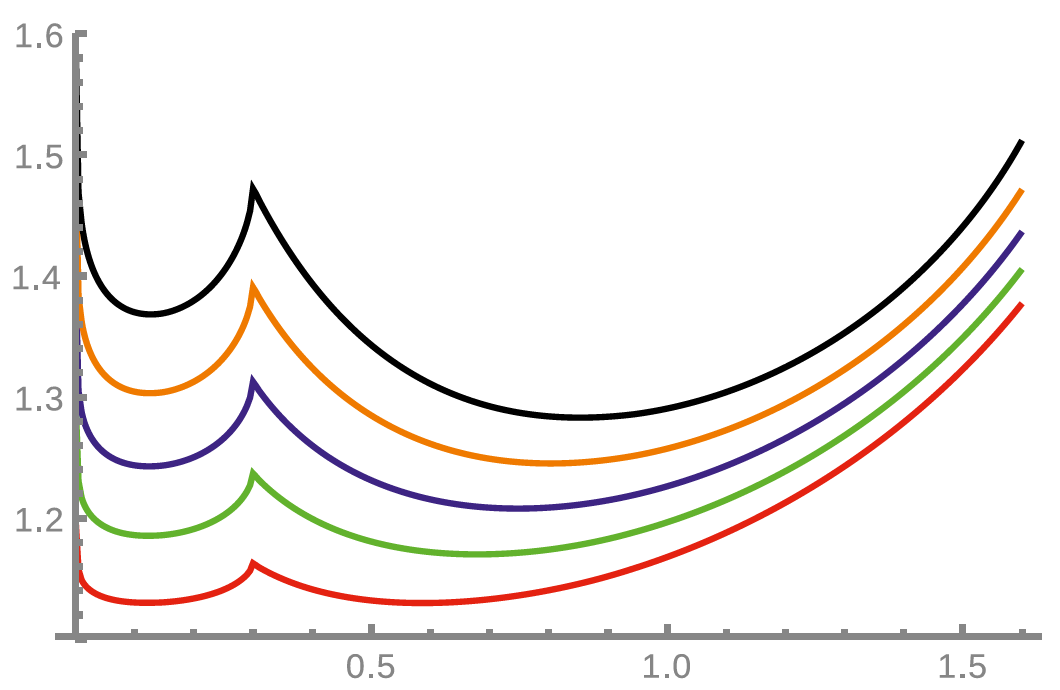
\includegraphics[scale = .25]{plot/3.png}
    \end{minipage}  
    \begin{minipage}[r]{.5\textwidth}
      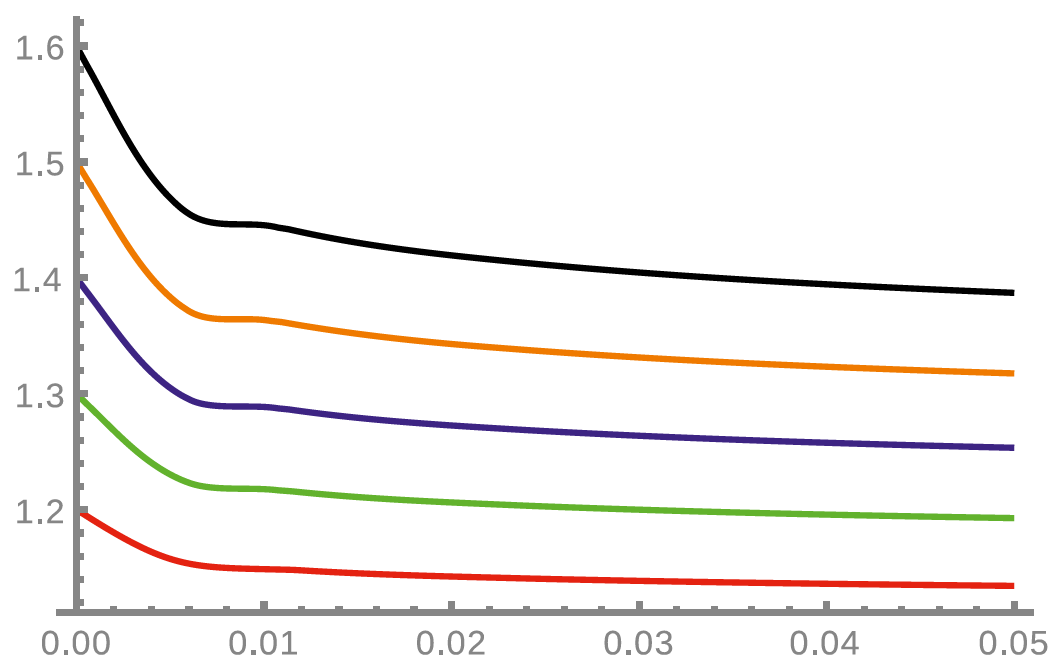
\includegraphics[scale = .25]{plot/4.png}
    \end{minipage} 
    \caption{
        Graphs of solutions to the differential equation $\leftindex[I]^C {D^{0.28}}y(t) = \sqrt{|0.3-t|} \sin(3y(t))+ 0.3t^3$
        with initial conditions $y(0) = 1.2$ (red), $y(0) = 1.3$ (green), $y(0) = 1.4$ (blue), $y(0) = 1.5$ (orange)
        and $y(0) = 1.6$ (black), plotted over the interval $[0, 1.6]$ (left) and zoom of this picture to the interval
        $[0, 0.05]$ (right). It can be observed that the graphs never meet or cross each other.
    } 
\end{figure*}
% \subsection{Terminal Value Problems For Single-Term Equations}
% A different type of problems has also received some attention recently
% Observing the state of the system at the point $t^*$ on the interval $[0, t^*]$, 
% Since the point $t^*$ at which the information is given is the end point of this interval, 
% a problem of this type is commonly referred to as a "terminal value problem".
% and it's the condition that accompany the equation is in the form of 
% \[
%     y(t^*) = \beta^*
% \]
% For the sake of simplicity, we restrict our attention to the case where one condition is imposed 
% which means we consider only differential equations of order $\alpha \in (0, 1)$, 
% now we need to see when such a terminal value problem have a unique solution. 

% If one can manage to find the solution on $[0, t^*]$ then the system's state at
% $t = 0$ is known and can be used to define a standard initial condition that then replaces
% the terminal condition, so that the new IVP can be solved on an interval
% $[0, T]$ with some $T > t^*$ 

% In the context of terminal value problems it suffices to work on the interval $[0, t^*]$. In
% this context, it is of interest to derive an analog of the integral equation formulation
% of the IVP that Lemma (6.1) provided. This result looks as follows.

% \begin{lemma}
%     Let $t^* > 0$ and $0 < \alpha < 1$, and assume $f := [0, t^*]\times \mathbb{R} \to \mathbb{R}$ to be continuous and
%     satisfies Lipschitz condition with respect to the second variable. Then the TVP
%     \begin{equation}
%         \begin{cases}
%             \leftindex[I]^C {D^{\alpha}} y(t) = f(t,y(t))
%             \\
%             T.C \Longrightarrow y(t^*) = \beta^*
%         \end{cases}
%     \end{equation}
%     Is equivalent to the weakly singular integral equation
%     \[
%         y(t) = \beta^* + \frac{1}{\Gamma(\alpha)}\int_{0}^{t^*} G(t,s)f(s,y(s)) \hquad ds
%     \]
%     Where 
%     \[
%         G(t,s)=
%         \begin{cases}
%             -(t^* - s)^{\alpha-1} & \text{ for } s>t
%             \\
%             (t-s)^{\alpha-1} - (t^* - s)^{\alpha-1} & \text{ for } s \leq t
%         \end{cases} 
%     \]
% \end{lemma}
% The substantial difference between the integral equation of Lemma (6.8) and the integral
% equation derived in Lemma (6.1) is that we now have a Fredholm integral equation of 
% Hammerstein type whereas the IVP gave rise to a Volterra equation. 

% Thus, in analogy with the corresponding results for integer order equations, 
% it would be natural to interpret the terminal condition as a boundary condition
% and not an initial condition. Hence, in contrast to the situation observed for
% first order differential equations, the TVP (6.6) is much more closely related to a boundary value problem than it is to an
% IVP.

% In spite of this difference, it is possible to provide an existence and uniqueness
% theorem for TVPs that formally coincides with the corresponding
% result for IVPs.
% \begin{theorem}
%     Under the assumptions of Lemma (6.8), the TVP (6.6) has exactly one continuous solution on $[0, t^*]$.
% \end{theorem}
% This result holds for the case of a scalar problem only, but not necessarily when
% the functions are assumed to be vector valued.

\newpage 

\subsection{Linear Fractional Differential Equations (LFDE)}
A linear FDE is an equation of form
\[
    \left(\leftindex[I]^C {D^{\alpha_m}} + a_{m-1}(t)\leftindex[I]^C {D^{\alpha_{m-1}}} + \dots + a_{1}(t)\leftindex[I]^C {D^{\alpha_{1}}} + a_{1}(t) \right) y(t) = f(t)
\]
With the conditions:
\[
    y^{(k)}(0) = \beta_k \quad,\quad k = 0,1,2,\dots,m-1
\]
\begin{theorem}[Existence And Uniqueness Of LFDE]
    If $f(t)$ is bounded on $(0, T)$ and $a_{k}(t)$ , $k = {0, 1, \dots , m-1}$ 
    are continuous functions on $[0, T]$, the equation has a unique solution.
\end{theorem}
In the particular case where the given differential equation is linear, it is often possible
to write up the solutions in closed form.
\begin{example}
    Show that 
    \[
        y(t) = \frac{1}{\Gamma(\alpha)}\int_{0}^{t} (t-s)^{\alpha-1}f(s) \hquad ds
    \]
    Solves the IVP 
    \[
        \begin{cases}
            \leftindex[I]^C {D^{\alpha}} y(t) = f(t)    \quad&,\quad m-1<\alpha<m
            \\
            I.C \Longrightarrow y^{(k)}(0) = 0 \quad&,\quad k = 0,1,2,\dots,m-1
        \end{cases}
    \]
    \textit{ \textbf{Sol.} } We apply the Laplace transform
        \begin{align*}
            \mathcal{L}\left[\leftindex[I]^C {D^{\alpha}} y(t)\right] &= \mathcal{L}[f(t)]
            \\
            s^{\alpha} Y(s) &= F(s)
            \\
            Y(s) &= s^{-\alpha}F(s)
            \\
            \mathcal{L}[y(t)] &= \mathcal{L}\left[I^{\alpha}f(t)\right]
            \\
            y(t) &= I^{\alpha}f(t) = \frac{1}{\Gamma(\alpha)}\int_{0}^{t} (t-s)^{\alpha-1}f(s) \hquad ds
        \end{align*}
\end{example}
\begin{enrichment*}{Laplace of Mittag Leffler Function }
    \[
        \mathcal{L}\left[t^{\beta-1} E_{\alpha,\beta}(\lambda t^\alpha)\right] = \frac{s^{\alpha - \beta}}{s^{\alpha}-\lambda}
    \]
\end{enrichment*}
\begin{example}
    Show that 
    \[
        y(t) = \sum_{k=0}^{m-1} \beta_k t^{k} E_{\alpha,k+1}(\lambda t^\alpha)
    \]
    Solves the IVP 
    \[
        \begin{cases}
            \leftindex[I]^C {D^{\alpha}} y(t) = \lambda y(t)    \quad&,\quad m-1<\alpha<m
            \\
            I.C \Longrightarrow y^{(k)}(0) = \beta_k \quad&,\quad k = 0,1,2,\dots,m-1
        \end{cases}
    \]
    \textit{ \textbf{Sol.} } We apply the Laplace transform
        \begin{align*}
            \mathcal{L}\left[\leftindex[I]^C {D^{\alpha}} y(t)\right] &= \lambda \mathcal{L}[y(t)]
            \\
            s^{\alpha} Y(s) - \sum_{k=0}^{m-1} s^{\alpha-k-1} y^{(k)}(0) &= \lambda Y(s)
            \\
            Y(s) &= \sum_{k=0}^{m-1} \frac{s^{\alpha-k-1}}{s^{\alpha}-\lambda} \beta_k
            \\
            \mathcal{L}[y(t)] &= \sum_{k=0}^{m-1} \mathcal{L}\left[\beta_k t^{k} E_{\alpha,k+1}(\lambda t^\alpha)\right]
            \\
            \mathcal{L}[y(t)] &= \mathcal{L}\left[\sum_{k=0}^{m-1} \beta_k t^{k} E_{\alpha,k+1}(\lambda t^\alpha)\right]
            \\
            y(t) &= \sum_{k=0}^{m-1} \beta_k t^{k} E_{\alpha,k+1}(\lambda t^\alpha)
        \end{align*}
\end{example}
In example (6.1.4) if we take special case when $m-1 = 0$ and for $\lambda = -1$. 
\[
    y(t) = \beta_0 E_{\alpha,1}(-t^\alpha)
\]
The cases $\alpha = 1$ and $\alpha = 2$
reduce to the well known statements that are the exponential function $E_{1,1}(-t) = e^{-t}$ and
the cosine $E_{2,1}(-t^2) = cos(t)$ solve the given first and second order IVPs.

This observation indicates that the solutions to the general problem of order $\alpha$ 
decay in a monotonic way for $\alpha = 1$ and exhibit persistent oscillations for $\alpha = 2$ if $\lambda$ is
a negative real number. 
And the behavior of the solution in the cases $1 < \alpha < 2$ and $0 < \alpha < 1$. 
The associated results are illustrated in Figure 2
\begin{figure*}[h]
    \begin{minipage}[l]{.5\textwidth}
      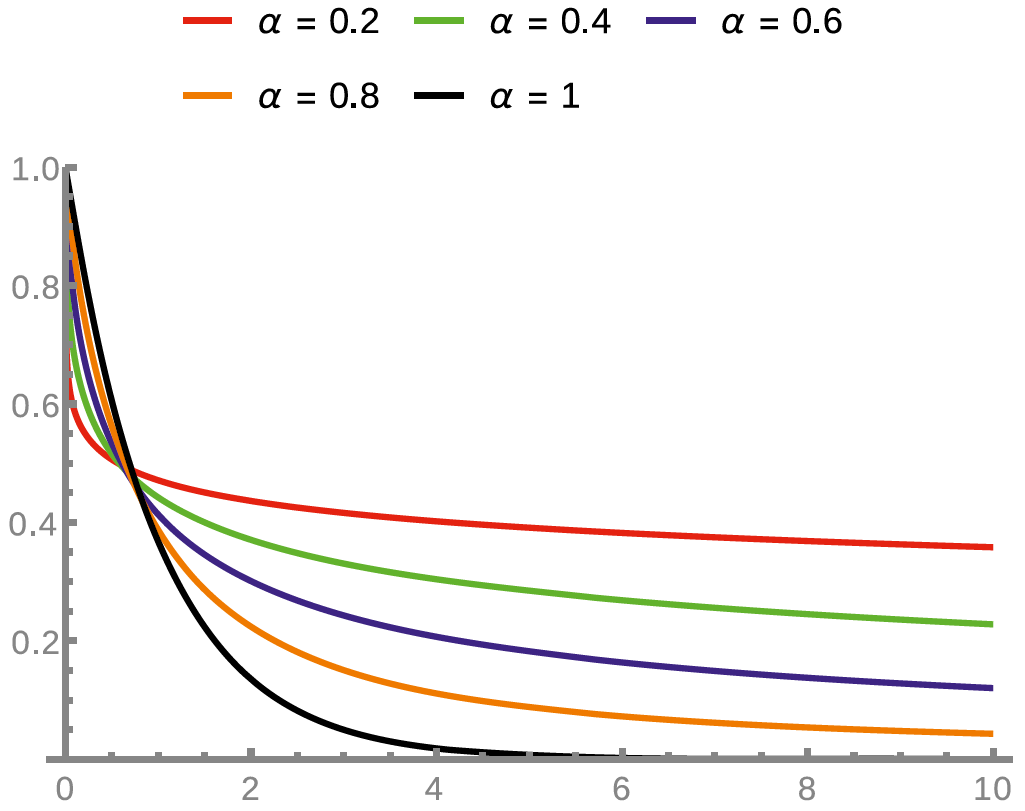
\includegraphics[scale = .25]{plot/1.png}
    \end{minipage}  
    \begin{minipage}[r]{.5\textwidth}
      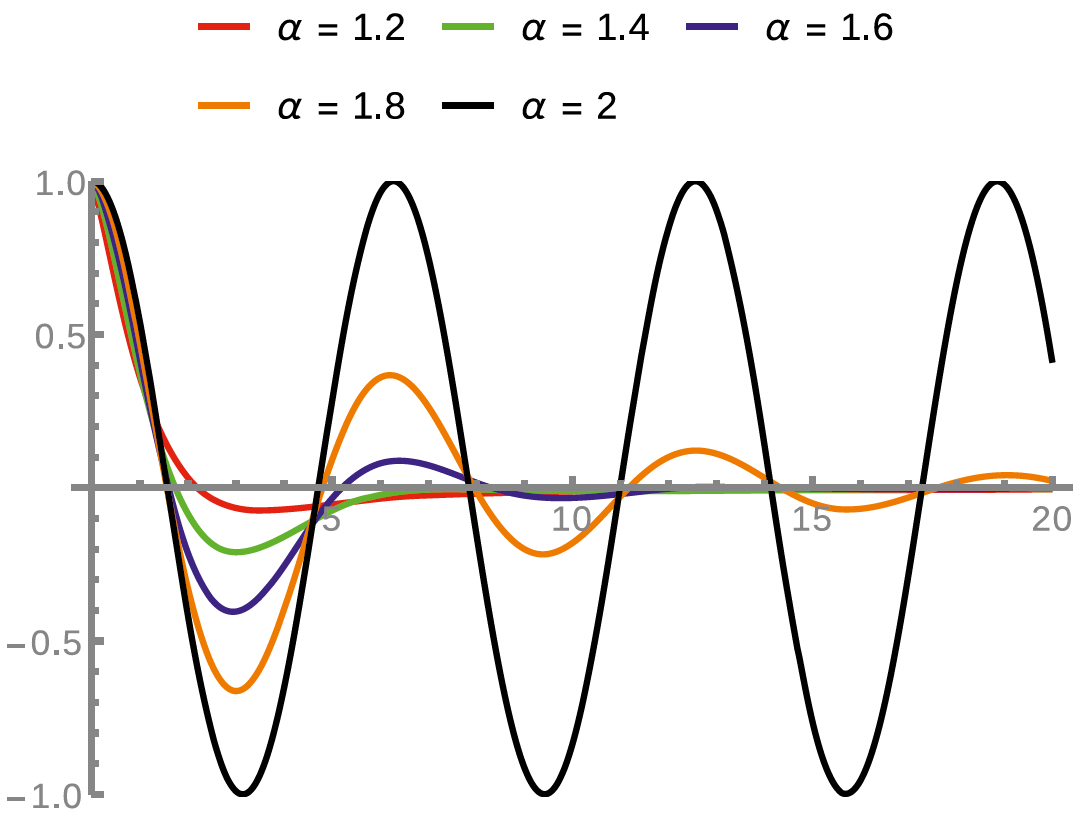
\includegraphics[scale = .25]{plot/2.png}
    \end{minipage} 
    \caption{Plots of $y(t) = E_{\alpha}(-t^\alpha)$ for various $\alpha \in (0, 1]$ (left) and $\alpha \in (1, 2]$ (right).} 
\end{figure*}

\begin{example}
    Show that 
    \[
        y(t) = \beta + t^{\alpha} \sum_{n=0}^{\infty} \frac{f^{(n)}(0)}{\Gamma(n+\alpha+1)}t^n
    \]
    Solves the IVP 
    \[
        \begin{cases}
            \leftindex[I]^C {D^{\alpha}} y(t) = f(t)    \quad,\quad 0<\alpha<1
            \\
            I.C \Longrightarrow y(0) = \beta
        \end{cases}
    \]
    \textit{ \textbf{Sol.} } We expand $f(t)$ using Taylor expansion and apply the Laplace transform
        \begin{align*}
            \mathcal{L}[\leftindex[I]^C {D^{\alpha}} y(t)] &= \mathcal{L}[f(t)]
            \\
            s^{\alpha} Y(s) - \beta s^{\alpha-1} &= \mathcal{L}\left[\sum_{n=0}^{\infty} \frac{f^{(n)}(0)}{\Gamma(n+1)}t^n\right]
            \\
            Y(s) &= \frac{\beta}{s} + \sum_{n=0}^{\infty} \frac{f^{(n)}(0)}{\Gamma(n+1)}\frac{1}{s^{\alpha}}\mathcal{L}[t^n]
            \\
            \mathcal{L}[y(t)] &= \mathcal{L}[\beta] + \sum_{n=0}^{\infty} \frac{f^{(n)}(0)}{\Gamma(n+1)}\frac{1}{s^{\alpha}}\frac{\Gamma(n+1)}{s^{n+1}}
            \\
            \mathcal{L}[y(t)] &= \mathcal{L}[\beta] + \sum_{n=0}^{\infty} f^{(n)}(0) \frac{1}{s^{n+\alpha+1}}
            \\
            \mathcal{L}[y(t)] &= \mathcal{L}[\beta] + \sum_{n=0}^{\infty} f^{(n)}(0) \mathcal{L}\left[\frac{t^{n+\alpha}}{\Gamma(n+\alpha+1)}\right]
            \\
            y(t) &= \beta + t^{\alpha} \sum_{n=0}^{\infty} \frac{f^{(n)}(0)}{\Gamma(n+\alpha+1)}t^n
        \end{align*}
\end{example}
% \newpage
\begin{example}
    Solve the in-homogeneous IVP 
    \[
        \begin{cases}
            \leftindex[I]^C {D^{\alpha}} y(t) = \lambda y(t) + Q(t)   \quad&,\quad m-1<\alpha<m
            \\
            I.C \Longrightarrow y^{(k)}(0) = \beta_k \quad&,\quad k = 0,1,2,\dots,m-1
        \end{cases}
    \]
    Where $Q \in C[0, h]$ is a given function 

    \textit{ \textbf{Sol.} } As we did previously we expand $Q(t)$ using Taylor expansion and apply the Laplace transform
    \begin{align*}
        \mathcal{L}\left[\leftindex[I]^C {D^{\alpha}} y(t)\right] &= \lambda \mathcal{L}[y(t)] + \mathcal{L}\left[\sum_{n=0}^{\infty} \frac{Q^{(n)}(0)}{\Gamma(n+1)}t^n\right]
        \\
        s^{\alpha} Y(s) - \sum_{k=0}^{m-1} s^{\alpha-k-1} y^{(k)}(0) &= \lambda Y(s) + \sum_{n=0}^{\infty} Q^{(n)}(0) s^{-n-1} 
        \\
        Y(s) &= \sum_{k=0}^{m-1} \frac{s^{\alpha-k-1}}{s^{\alpha}-\lambda} \beta_k + \sum_{n=0}^{\infty} Q^{(n)}(0) \frac{s^{-n-1} }{s^{\alpha}-\lambda}
        \\
        \mathcal{L}[y(t)] &= \sum_{k=0}^{m-1} \mathcal{L}\left[\beta_k t^{k} E_{\alpha,k+1}(\lambda t^\alpha)\right] + \sum_{n=0}^{\infty} Q^{(n)}(0) \frac{s^{\alpha-\alpha-n-1} }{s^{\alpha}-\lambda}
        \\
        \mathcal{L}[y(t)] &= \mathcal{L}\left[\sum_{k=0}^{m-1} \beta_k t^{k} E_{\alpha,k+1}(\lambda t^\alpha)\right] + \sum_{n=0}^{\infty} \mathcal{L}\left[Q^{(n)}(0) t^{\alpha+n} E_{\alpha,\alpha+n+1}(\lambda t^\alpha)\right]
        \\
        \mathcal{L}[y(t)] &= \mathcal{L}\left[\sum_{k=0}^{m-1} \beta_k t^{k} E_{\alpha,k+1}(\lambda t^\alpha)\right] + \mathcal{L}\left[\sum_{n=0}^{\infty} Q^{(n)}(0) t^{\alpha+n} E_{\alpha,\alpha+n+1}(\lambda t^\alpha)\right]
        \\
        \tag{6.7} y(t) &= \sum_{k=0}^{m-1} \beta_k t^{k} E_{\alpha,k+1}(\lambda t^\alpha) + \sum_{n=0}^{\infty} Q^{(n)}(0) t^{\alpha+n} E_{\alpha,\alpha+n+1}(\lambda t^\alpha)
        \intertext{Using Mittag Leffler function recursion relation $\displaystyle E_{\alpha,\alpha+\beta}(z) = \frac{1}{z}\left[E_{\alpha,\beta}(z) - \frac{1}{\Gamma(\beta)}\right]$}
        &= \sum_{k=0}^{m-1} \beta_k t^{k} E_{\alpha,k+1}(\lambda t^\alpha) + \sum_{n=0}^{\infty} Q^{(n)}(0) t^{\alpha+n} \frac{1}{\lambda t^\alpha}\left[E_{\alpha,n+1}(z) - \frac{1}{\Gamma(n+1)}\right]
        \\
        &= \sum_{k=0}^{m-1} \beta_k t^{k} E_{\alpha,k+1}(\lambda t^\alpha) + \frac{1}{\lambda}\sum_{n=0}^{\infty} Q^{(n)}(0) t^{n}E_{\alpha,n+1}(z) - \frac{Q(t)}{\lambda}
        \setcounter{equation}{7}
    \end{align*}
Another way using the superposition principle
\begin{enrichment*}{The Superposition Principle}
    The solution of the in-homogeneous equation can be written as the 
    sum of the solution of the homogeneous equation, and a particular 
    solution of the in-homogeneous equation.
\end{enrichment*}
We can break the problem into the following two problems
\[
    \begin{cases}
        \leftindex[I]^C {D^{\alpha}} y_h(t) = \lambda y_h(t)  \quad&,\quad m-1<\alpha<m
        \\
        I.C \Longrightarrow y_h^{(k)}(0) = \beta_k \quad&,\quad k = 0,1,2,\dots,m-1
    \end{cases}
\]
\[
    \begin{cases}
        \leftindex[I]^C {D^{\alpha}} y_p(t) = \lambda y_p(t) + Q(t)   \quad&,\quad m-1<\alpha<m
        \\
        I.C \Longrightarrow y_p^{(k)}(0) = 0 \quad&,\quad k = 0,1,2,\dots,m-1
    \end{cases}
\]
Where $y = y_h + y_p$ solves the original problem.
From example (6.3.2) we got that
\[
    y_h(t) = \sum_{k=0}^{m-1} \beta_k t^{k} E_{\alpha,k+1}(\lambda t^\alpha)
\]
Now for the second problem take Laplace Transform for it 
\begin{align*}
    \mathcal{L}\left[\leftindex[I]^C {D^{\alpha}} y_p(t)\right] &= \lambda \mathcal{L}[y_p(t)] + \mathcal{L}\left[\sum_{n=0}^{\infty} \frac{Q^{(n)}(0)}{\Gamma(n+1)}t^n\right]
    \\
    s^{\alpha} Y_p(s) &= \lambda Y_p(s) + \sum_{n=0}^{\infty} Q^{(n)}(0) s^{-n-1} 
    \\
    Y_p(s) &= \sum_{n=0}^{\infty} Q^{(n)}(0) \frac{s^{-n-1} }{s^{\alpha}-\lambda} = \sum_{n=0}^{\infty} Q^{(n)}(0) \frac{s^{\alpha-\alpha-n-1} }{s^{\alpha}-\lambda}
    \\
    \mathcal{L}[y_p(t)] &= \sum_{n=0}^{\infty} \mathcal{L}\left[Q^{(n)}(0) t^{\alpha+n} E_{\alpha,\alpha+n+1}(\lambda t^\alpha)\right]
    \\
    \mathcal{L}[y_p(t)] &= \mathcal{L}\left[\sum_{n=0}^{\infty} Q^{(n)}(0) t^{\alpha+n} E_{\alpha,\alpha+n+1}(\lambda t^\alpha)\right]
    \\
    y_p(t) &= \sum_{n=0}^{\infty} Q^{(n)}(0) t^{\alpha+n} E_{\alpha,\alpha+n+1}(\lambda t^\alpha)
\end{align*}
Adding $y_h + y_p$ we get the result (6.7)
\end{example}
\begin{enrichment*}{Duhamel's Principle}
    If one can solve an IVP for a homogeneous linear differential equation then an in-homogeneous linear differential equation can be solved as well.
\end{enrichment*} 
\newpage
\subsection{Nonlinear Equations}
Now we will discuss One of the methods to solve Nonlinear FDE which is The Adomian Decomposition Method

The Adomian method applied to the ordinary and partial differential equations of integer order was extended 
also to the case of FDE.
\subsubsection{The Adomian Decomposition Method (ADM)}
Before we talk about how to solve FDE using ADM let us first see how it work 

Consider the problem
\begin{equation}
    \begin{cases}
        \displaystyle \pdv{u(x,t)}{t} + L(u(x,t)) + N(u(x,y)) = g(x,t)
        \\
        I.C \Longrightarrow \displaystyle u(x,0) = \phi(x)
    \end{cases}
\end{equation}
This is nonlinear partial differential equation of integer order where $L(u(x,t))$ is the linear part and $N(u(x,t))$ is the non-linear part
We will discuss it's solution by ADM
\\
Now, Integrate (6.8) from $0 \to t$
\begin{equation}
    u(x,t) = \phi(x) - \int_{0}^{t} L(u(x,s)) \hquad ds  - \int_{0}^{t} N(u(x,s)) \hquad ds  + \int_{0}^{t} g(x,s) \hquad ds
\end{equation}
Set
\begin{equation}
    u(x,t) = \sum_{n=0}^{\infty} u_n(x,y)
\end{equation}
\begin{equation}
    N(u(x,t)) = \sum_{n=0}^{\infty} A_n(x,y)
\end{equation}
Where $A_0,A_1,A_2,\dots$ are \textbf{Adomian Polynomials} defined as:
\[
    A_n(x,y) = \frac{1}{n!} \dv[n]{}{\lambda} \left( N \left( \sum_{j=0}^{n}\lambda^j u_j \right) \right)
\]
Substitute equations (6.10),(6.11) into (6.9) we get
\begin{equation*}
    u(x,y) = \sum_{n=0}^{\infty}u_n(x,t) = \phi(x) + \int_0^t g(x,s) \hquad ds - \int_0^t L \left(\sum_{n=0}^{\infty}u_n(z,t)\right)  - \int_0^t \sum_{n=0}^{\infty}A_n(x,s) \hquad ds
\end{equation*}
Now,
\begin{align*}
    u_0 & = \phi(x) + \int_0^t g(x,s) \hquad ds                 \\
    u_1 & = -\int_0^t L(u_0) \hquad ds - \int_0^t A_0 \hquad ds         \\
    u_2 & = -\int_0^t L(u_1) \hquad ds - \int_0^t A_1 \hquad ds         \\
    \vdots                                               \\
    u_n & = -\int_0^t L(u_{n-1}) \hquad ds - \int_0^t A_{n-1} \hquad ds
\end{align*}
\[
    \therefore u(x,t) = \sum_{n=0}^{\infty} u_n(x,y) = u_0 + u_1 + u_2 + \dots
\]
This will get the solution for the problem (6.8)
\newpage
Note that The Adomian Decomposition Method (ADM)
is a numerical technique used to approximate solutions
of differential equations.
Whether ADM converges or diverges depends on the
specific problem and how it is applied.
The convergence and divergence of ADM can be
influenced by several factors, including the
complexity of the problem, the choice of the
decomposition functions, and the behavior of
the nonlinear terms in the differential equation.

\begin{example}
    Solve the nonlinear differential equation using ADM
    \begin{equation}
        \begin{cases}
            \displaystyle \frac{\partial u(x,t)}{\partial t} = x^2 - \frac{1}{4}\left( \frac{\partial u(x,t)}{\partial x} \right)^2
            \\
            I.C \Longrightarrow \displaystyle u(x,0) = 0
        \end{cases}
    \end{equation}
    \textit{ \textbf{Sol.} } Set
    \begin{align*}
        u(x,t) & = \sum_{n=0}^{\infty} u_n(x,t)
        \\
        N(u)   & = \sum_{n=0}^{\infty} A_n(x,t)
    \end{align*}
    Where $N(u)$ represents the nonlinear form of $u$ 
    
    In our case in equation (6.12) $\displaystyle N(u) = \left(\frac{\partial u}{\partial x}\right)^2$
    \begin{align*}
        A_n(x,t) & = \left[\frac{1}{n!} \frac{d^n}{d \lambda^n} N\left(\sum_{i=0}^{n}  \lambda^i u_i(x,t)\right)\right]_{\lambda = 0}
        \\
        A_n(x,t) & = \left[\frac{1}{n!} \frac{d^n}{d \lambda^n} \left(\sum_{i=0}^{n}  \lambda^i \frac{\partial u_i(x,t)}{\partial x}\right)^2\right]_{\lambda = 0}
    \end{align*}
    Integrating equation (6.12) from $0 \to t$
    \[
        u(x,t) = \sum_{n=0}^{\infty} u_n(x,t)  = x^2t - \frac{1}{4} \int_{0}^{t}\sum_{n=0}^{\infty} A_n(x,\theta) \hquad d\theta
    \]
    Now we get $A_0$,$A_1$,$A_2,\dots$
    \begin{align*}
        A_0(x,\theta) & = \left[\sum_{i=0}^{0}  \lambda^i \frac{\partial u_i(x,\theta)}{\partial x}^2\right]_{\lambda = 0} = \left(\frac{\partial u_0(x,\theta)}{\partial x}\right)^2
        \\
        A_1(x,\theta) & = \left[\frac{d}{d \lambda} \left(\sum_{i=0}^{1}  \lambda^i \frac{\partial u_i(x,\theta)}{\partial x}\right)^2\right]_{\lambda = 0}
        \\
                      & = \left[\frac{d}{d \lambda} \left(\frac{\partial u_0(x,\theta)}{\partial x} + \lambda \frac{\partial u_1(x,\theta)}{\partial x}\right)^2\right]_{\lambda = 0}
        \\
                      & =2\left[\left(\frac{\partial u_0(x,\theta)}{\partial x} + \lambda \frac{\partial u_1(x,\theta)}{\partial x}\right)\frac{\partial u_1(x,\theta)}{\partial x}\right]_{\lambda = 0} = 2\frac{\partial u_0(x,\theta)}{\partial x} \frac{\partial u_1(x,\theta)}{\partial x}
        \\
        A_2(x,\theta) & =\left[\frac{1}{2!} \frac{d^2}{d \lambda^2} \left(\sum_{i=0}^{2}  \lambda^i \frac{\partial u_i(x,\theta)}{\partial x}\right)^2\right]_{\lambda = 0}
        \\
                      & = \left[\frac{1}{2} \frac{d^2}{d \lambda^2} \left(\frac{\partial u_0(x,\theta)}{\partial x} + \lambda \frac{\partial u_1(x,\theta)}{\partial x} + \lambda^2 \frac{\partial u_2(x,\theta)}{\partial x}\right)^2\right]_{\lambda = 0}
        \\
                      & = \left(\frac{\partial u_1(x,\theta)}{\partial x}\right)^2 + 2 \left(\frac{\partial u_0(x,\theta)}{\partial x}\frac{\partial u_2(x,\theta)}{\partial x}\right)
        \\
        A_3(x,\theta) & = 2\frac{\partial u_1(x,\theta)}{\partial x}\frac{\partial u_2(x,\theta)}{\partial x} + 2\frac{\partial u_0(x,\theta)}{\partial x} \frac{\partial u_3(x,\theta)}{\partial x}
    \end{align*}
    Now because
    \[
        u_0 + u_1 + u_2 + \dots = u(x,t) = x^2t - \frac{1}{4}\int_{0}^{t}[A_0+A_1+A_2+\dots] \hquad d\theta
    \]
    Then
    \begin{align*}
        u_0 & = x^2t
        \\
        u_1 & = -\frac{1}{4}\int_{0}^{t}A_0d\theta = -\frac{1}{4}\int_{0}^{t}\left(\frac{\partial u_0(x,\theta)}{\partial x}\right)^2 = -\int_{0}^{t} x^2 \theta^2 d\theta = \frac{-1}{3}x^2t^3
        \\
        u_2 & = \frac{2}{15} x^2t^5
        \\
        u_3 &= \frac{-17}{315} x^2t^7 
        \\
        \vdots
    \end{align*}
    \[
        u(x,t) = x^2 \left[t-\frac{1}{3}t^3 + \frac{2}{15} t^5 - \frac{17}{315} t^7 \dots\right] = x^2 \tanh(t)
    \]
\end{example}
\begin{figure}[b]
    \begin{enrichment}{George Adomian}{Chars/adom.jpg}{2.4}{.8}{.17}
        George Adomian (March 21, 1922 – June 17, 1996)
        was an American mathematician of Armenian descent
        who developed the Adomian decomposition method (ADM)
        for solving nonlinear differential equations,
        both ordinary and partial.
        The method is explained among other places
        in his book \textit{\textbf{"Solving Frontier Problems in Physics:
                The Decomposition Method"}}.
        He was a faculty member at the University of Georgia
        (UGA) from 1966 through 1989. While at UGA,
        he started the Center for Applied Mathematics.
        Adomian was also an aerospace engineer.
    \end{enrichment}
\end{figure}
\newpage
\subsubsection{Decomposition Of Nonlinear FDE}
We consider the following nonlinear FDE 
\begin{equation}
    \begin{cases}
        \displaystyle \leftindex[I]^C {D^{\alpha}} y(t) + L(y(t)) + N(y(t)) = f(t)
        \\
        I.C \Longrightarrow \displaystyle y^{(k)}(0) = \beta_k \quad,\quad k=0,1,2,\dots,m-1 
    \end{cases}
\end{equation}
We apply the Laplace Transform to the equation
\[
    \mathcal{L}[\leftindex[I]^C {D^{\alpha}} y(t)] = s^{\alpha} Y(s) - \sum_{k=0}^{m-1} s^{\alpha-k-1} y^{(k)}(0)
\]
We use the following decomposition of $y(t)$
\[
    y(t) = \sum_{n=0}^{\infty} y_n(t)
\]
And 
\[
    N(y(t)) = \sum_{n=0}^{\infty} A_n
\]
Where $A_n$ are Adomian polynomials

The equation (6.13) become 
\[
    \mathcal{L}\left[\sum_{n=0}^{\infty} y_n(t)\right] = \sum_{k=0}^{m-1} \frac{\beta_k}{s^{k+1}} - \frac{1}{s^{\alpha}} \mathcal{L}\left[L\left(\sum_{n=0}^{\infty} y_n(t)\right)\right] - \frac{1}{s^{\alpha}}\mathcal{L}\left[\sum_{n=0}^{\infty} A_n\right] + \frac{1}{s^{\alpha}}\mathcal{L}\left[f(t)\right]
\]
Now we can get 
\begin{align*}
    Y_0 &= \mathcal{L}\left[y_0\right] = \sum_{k=0}^{m-1} \frac{\beta_k}{s^{k+1}} + \frac{1}{s^{\alpha}}\mathcal{L}\left[f(t)\right]
    \\
    Y_1 &= \mathcal{L}\left[y_1\right] = - \frac{1}{s^{\alpha}} \mathcal{L}\left[L\left(y_0(t)\right)\right] - \frac{1}{s^{\alpha}}\mathcal{L}\left[ A_0\right]
    \\
    Y_2 &= \mathcal{L}\left[y_2\right] = - \frac{1}{s^{\alpha}} \mathcal{L}\left[L\left(y_1(t)\right)\right] - \frac{1}{s^{\alpha}}\mathcal{L}\left[ A_1\right]
    \\
    \vdots
    \\
    Y_n &= \mathcal{L}\left[y_n\right] = - \frac{1}{s^{\alpha}} \mathcal{L}\left[L\left(y_{n-1}(t)\right)\right] - \frac{1}{s^{\alpha}}\mathcal{L}\left[ A_{n-1}\right]
\end{align*}
\begin{example}
    Solve the nonlinear FDE using the Adomian decomposition method
    \[
        \begin{cases}
            \displaystyle \leftindex[I]^C {D^{\alpha}} y(t) = t + y^2 \quad,\quad 1<\alpha \leq 2
            \\
            I.C \Longrightarrow \displaystyle y(0) = 0 \quad,\quad y^{(1)}(0) = 1
        \end{cases}
    \]
    \textit{ \textbf{Sol.} } In order to solve the equation we apply the Laplace transform
    \begin{align*}
        \mathcal{L}\left[\leftindex[I]^C {D^{\alpha}} y(t)\right] &= \mathcal{L}\left[t + y^2\right]
        \\
        s^{\alpha} Y(s) - s^{\alpha-1}y(0) - s^{\alpha-2} y^{(1)}(0) &= \mathcal{L}\left[t + y^2\right]
        \\
        s^{\alpha} Y(s) - s^{\alpha-2} &= \mathcal{L}\left[t + y^2\right]
    \end{align*}
    So that, for the decomposition
    \[
        y(t) = \sum_{n=0}^{\infty} y_n(t)
    \]
    We obtain
    \[
        Y(s) = \sum_{n=0}^{\infty} Y_n(s) \quad , \quad t+y^2 = \sum_{n=0}^{\infty} A_n
    \]
    The Adomian polynomials $A_n$ are 
    \[
        A_0 = t + y_0^2 \quad,\quad A_1 = 2y_0y_1 \quad,\quad A_2 = y_1^2 + 2y_0y_2 \quad,\quad A_2 = 2y_1y_2 + 2y_0y_3 \quad,\dots
    \]
    \[
        Y_0 = \frac{1}{s^2} \quad\Longrightarrow\quad y_0 = t \quad\Longrightarrow\quad A_0 = t+t^2
    \]
    \[
        Y_1 = \frac{1}{s^\alpha}\mathcal{L}\left[A_0\right] \quad\Longrightarrow\quad y_1 = \frac{t^{\alpha+1}}{\Gamma(\alpha+2)} + 2\frac{t^{\alpha+2}}{\Gamma(\alpha+3)} \quad\Longrightarrow\quad A_1 = 2y_0y_1
    \]
    And so on 
    \[
        y(t) = y_0 + y_1 + y_2 + \dots
    \]
\end{example}


\subsection{Fractional Systems of Differential Equations}
Solving System of FDE is not very different from solving single FDE 
there are Linear Systems which can be solved using Laplace Transform 
and we will show example of them and there are Nonlinear Systems
which can be solved by Method of Successive Approximations and
The Adomian Decomposition Method

\begin{example}
    Solve the system of FDE
    \[
        \begin{cases}
            \displaystyle \leftindex[I]^C {D^{\alpha}} x(t) = \leftindex[I]^C {D^{\beta}} y(t) + 1  \quad,\quad 0<\alpha<1
            \\
            \displaystyle \leftindex[I]^C {D^{\beta}} y(t) = 2\leftindex[I]^C {D^{\alpha}} x(t) - 1 \quad,\quad 0<\beta<1
            \\
            I.C \Longrightarrow x(0) = 1 \quad,\quad y(0) = 1
        \end{cases}
    \]
    \textit{ \textbf{Sol.} } We apply the Laplace Transform method
    \[
        \begin{cases}
            \displaystyle \mathcal{L}\left[\leftindex[I]^C {D^{\alpha}} x(t) \right]= \mathcal{L}\left[\leftindex[I]^C {D^{\beta}} y(t)\right] + \mathcal{L}\left[1\right]
            \\
            \displaystyle \mathcal{L}\left[\leftindex[I]^C {D^{\beta}} y(t) \right]= 2\mathcal{L}\left[\leftindex[I]^C {D^{\alpha}} x(t)\right] - \mathcal{L}\left[1\right]
        \end{cases}
    \]
    We obtain the system
    \[
        \begin{cases}
            \displaystyle s^\alpha X(s) - s^{\alpha-1} = s^\beta Y(s) - s^{\beta-1} + \frac{1}{s}
            \\
            \displaystyle s^\beta Y(s) - s^{\beta-1} = 2s^\alpha X(s) - 2s^{\alpha-1} - \frac{1}{s}
        \end{cases}
    \]
    With the solution:
    \[
        \begin{cases}
            \displaystyle X(s) = \frac{1}{s}
            \\\\
            \displaystyle Y(s) = \frac{1}{s} - \frac{1}{s^{\beta+1}}
        \end{cases}
    \]
    Take the Laplace inverse we get the solution for the original system
    \[
        \begin{cases}
            \displaystyle x(t) = 1 
            \\\\
            \displaystyle y(t) = 1 - \frac{t^{\beta}}{\Gamma(\beta+1)}
        \end{cases}
    \]
\end{example}